\documentclass[12pt]{article}
%\usepackage{html}
\usepackage{hyperref}
\usepackage{graphicx}
\title{CS 571\\Homework 2 Solution}
%\addtolength{\topmargin}{-2cm}
%\addtolength{\topskip}{-2cm}
%\addtolength{\oddsidemargin}{-2cm}
%\addtolength{\evensidemargin}{-2cm}
%\addtolength{\textheight}{2cm}
%\addtolength{\textwidth}{2cm}
%\addtolength{\footskip}{-1cm}
\date{}
\begin{document}
\maketitle

\begin{flushleft}
\textbf{Due}: Oct 19\hfill\textbf{100 points}\\

\textbf{No Late Submissions}

\vspace{0.5cm}

\textbf{Important Reminder}: As per the course Academic Honesty
Statement, cheating of any kind will minimally result in receiving an
F letter grade for the entire course.

\vspace{0.5cm}
To be submitted on paper in class.

\end{flushleft}

\begin{enumerate}

\item On a particular 32-bit architecture, a stack frame for a
  function with \verb@n@ parameters and \verb@m@ local variables is laid
  out as follows:

  Parameter \verb@n@ at offset \verb@4 * (n + 1)@ from the frame-pointer\\
  ...\\
  Parameter 1 at offset \verb@8@ from the frame-pointer\\
  Return address at offset \verb@4@ from the frame-pointer\\
  Saved frame-pointer at offset \verb@0@ from the frame-pointer\\
  Local variable 1 at offset \verb@-4@ from the frame-pointer\\
  Local variable 2 at offset \verb@-8@ from the frame-pointer\\
  ...\\
  Local variable \verb@m@ at offset \verb@-4*m@ from the frame-pointer.

  Assuming that the stack-frame contains only the above:

  \begin{enumerate}
  \item Give a formula in terms of \verb@n@ and \verb@m@ for the size
    (in bytes) of a stack-frame.

  \item Given the function

\begin{verbatim}
     f(int a, int b, int c) { //parameters a, b, c
       var d, e, f, g;        //local vars d, e, f, g.
        ...
     }
  \end{verbatim}
     Show the layout of the stack-frame for an invocation of f; Your
 answer should include the offset from the frame-pointer of each parameter
and local variable. \hfill{\textit{15-points}}


    \end{enumerate}

\begin{enumerate}

\item The \verb@n@ parameters occupy \verb@4 * n@ bytes; the \verb@m@
 local variables occupy \verb@4 * m@ bytes; the saved frame-pointer
 and return address occupy 4 bytes each.  Hence the total is
 \verb@4 * (n + m + 2)@ bytes.

\item The stack-frame will be laid out as follows:
\begin{verbatim}
                 +-------------------+
              16 |       c           |
                 +-------------------+
              12 |       b           |
                 +-------------------+
               8 |       a           |
                 +-------------------+
               4 |  return address   |
                 +-------------------+
    current--> 0 |saved frame pointer|
 frame pointer   +-------------------+
              -4 |       d           |
                 +-------------------+
              -8 |       e           |
                 +-------------------+
             -12 |       f           |
                 +-------------------+
             -16 |       g           |
                 +-------------------+
\end{verbatim}
\end{enumerate}

\item Given the following program in a statically-scoped language
 which supports nested functions:

\begin{verbatim}
f(a, b) {                 //1

  var x = ...;            //2

  g(a, x) {               //3
    var x = ...;          //4

    h(b) {                //5
      var a = ...;        //6
      return a + b*x;     //refs to a, b, x.
    }
  
    //body of g()
    return b + h(a)*x;    //refs to a, b, x.
  }

  //body of f()
  return a*b + x;         //refs to a, b, x.
}
\end{verbatim}

Local variable declarations are indicated using \verb@var@.  Points
$i$ where variables are defined are indicated using a comment
\verb@//@$i$.

For each line above which contains a comment \verb@refs to a, b, x@,
for each referenced variable show which declaration it refers to.
\hfill{\textit{15-points}}

\begin{tabular}{|l||c|c|c|}
  \hline
  Expression & \verb@a@ Declaration & \verb@b@ Declaration & \verb@x@ Declaration \\
  \hline
  \verb@a + b*x@ & \verb@//6@ & \verb@//5@ & \verb@//4@\\
  \verb@b + h(a)*x@ & \verb@//3@ & \verb@//1@ & \verb@//4@\\
  \verb@a*b + x@ & \verb@//1@ & \verb@//1@ & \verb@//2@\\
  \hline
\end{tabular}

\item Given the following program in a language which supports
 first-class functions as well as both lexically-scoped (indicated
 using a \verb@lex@ declaration) and dynamically-scoped variables
 (indicated using a \verb@dyn@ declaration) with \verb@lambda@ used to
 define anonymous functions.

\begin{verbatim}
//declare dynamically scoped var
dyn b = 3;

//Define function f with single parameter a
f(a) {
  lex static1 = a * 2; 
  lex static2 = b; 
  //return function which takes a single parameter x.
  return lambda (x) { return x + static1*static2 + b; }
}

//Define function f with single parameter a
sub h(a) {
  dyn b = a + 5
  return f(5)
}

//print result of calling return'd function from h(3) with 
//actual parameter 5.
print h(3)(5);

\end{verbatim}

What will be printed by the above program?  Justify your answer by showing the
values of all the variables.  \hfill{\textit{15-points}}

Annotating the program to show values of variables:

\begin{verbatim}
dyn b = 3;

f(a) {                        //f(5) called; hence a == 5
  lex static1 = a * 2;        //static1 = 5 * 2; hence static1 == 10
  lex static2 = b;            //static2 = value of b in caller h(); 
                              //hence static2 == 8
  //returns (lambda (x) { return x + 10*8 + b })
  return lambda (x) { return x + static1*static2 + b; }
}

sub h(a) {                    //h(3) called; hence a == 3
  dyn b = a + 5               //b = 3 + 5; hence b ==  8
  return f(5)
}

//h() returns above lambda value, which is then called with parameter 5
//i.e. (lambda (x) { return x + 10*8 + b })(5)
//Since h() has returned, b reverts to 3.
//Hence the above lambda reduces to 5 + 10*8 + 3 == 88
print h(3)(5);                //88 is printed.
\end{verbatim}

Note that Perl supports both lexical and dynamic variables as well as
nested anonymous functions.  The \href{./lex-dyn.pl}{lex-dyn.pl} program shows
a translation of the above program into Perl syntax.

\item Consider the tree structure shown in the figure below (taken from the \href{http://zdu.binghamton.edu/cs571-16f/slides/scheme/scheme.pdf}{Scheme Slides}).

  \begin{center}
    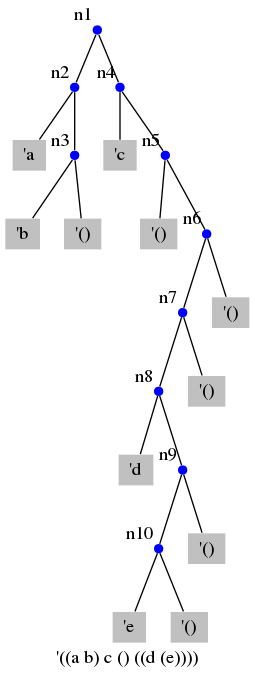
\includegraphics[height=120mm]{nest2}\\
  \end{center}

  By providing the Scheme expression equivalent to the subtree rooted
  at each internal node \verb@n1@ $\ldots$ \verb@n10@, show that the
  root node \verb@n1@ is equivalent to \verb@'((a b) c () ((d (e))))@.
  \hfill{\textit{15-points}}

  Filling in the values of the internal nodes using a bottom-up
  traversal of the tree, we have:

  \begin{eqnarray*}
    \mbox{\texttt{n10}} & = & \mbox{\texttt{'(e)}} \\
    \mbox{\texttt{n9}} & = & \mbox{\texttt{'((e))}} \\
    \mbox{\texttt{n8}} & = & \mbox{\texttt{'(d (e))}} \\
    \mbox{\texttt{n7}} & = & \mbox{\texttt{'((d (e)))}} \\
    \mbox{\texttt{n6}} & = & \mbox{\texttt{'(((d (e))))}} \\
    \mbox{\texttt{n5}} & = & \mbox{\texttt{'( () ((d (e))))}} \\
    \mbox{\texttt{n4}} & = & \mbox{\texttt{'( c () ((d (e))))}} \\
    \mbox{\texttt{n3}} & = & \mbox{\texttt{'(b)}} \\
    \mbox{\texttt{n2}} & = & \mbox{\texttt{'(a b)}} \\
    \mbox{\texttt{n1}} & = & \mbox{\texttt{'( (a b) c () ((d (e))))}} 
  \end{eqnarray*}

Hence the root is indeed equal to \verb@'( (a b) c () ((d (e))))@.
  
\item Show that the \verb@count-non-pairs@ function discussed in the
  \href{http://zdu.binghamton.edu/cs571-16f/slides/scheme/scheme.pdf}{Scheme Slides} will always terminate. 

(Termination is usually shown by identifying some quantity which
  cannot go below some value and showing that the quantity decreases
  as the computation progresses. Since the quantity cannot decrease
  below the minimum bound, the computation must
  terminate). \hfill{\textit{10-points}}

  The \verb@count-non-pairs@ function code was given as:

\begin{verbatim}
(define (count-non-pairs ls)
  (if (not (pair? ls))
      1
      (+ (count-non-pairs (car ls))
	    (count-non-pairs (cdr ls)))))
\end{verbatim}

Termination can be shown by arguing that the depth of the argument
decreases on each recursive call.  Specifically, define 
$\mbox{depth}(t)$ of a Scheme term $t$ as follows:
\begin{itemize}
\item If $t$ is not a pair, then $\mbox{depth}(t)$ is 0.
  \item If $t$ is a pair, then $\mbox{depth}(t)$ is $1 + \max($\mbox{depth}(\mbox{\texttt{car}}(t))), $\mbox{depth}(\mbox{\texttt{cdr}}(t))))$
\end{itemize}

Hence for the first recursive call above, it is clear that the depth
of the argument \verb@(car ls)@ is less than the depth of the incoming
argument \verb@ls@.  Similary, for the second recursive call above, it
is clear that the depth of the argument \verb@(cdr ls)@ is less than
the depth of the incoming argument \verb@ls@.

Since the size of the argument for each recursive call is strictly
smaller than the size of the incoming argument, the function must
terminate.

\item How would you build conceptually infinite lists in a language
  like Scheme.  

  Specifically, if you are given

\begin{description}

\item[\texttt(next v)] 
A function which generates the next element
 in the list when given the value \verb@v@ of the previous element in
 the list.

\item[\texttt{init}] 
 A value representing the first element in the list.
\end{description}

  describe how you would build a
  data-structure which acts like an infinite list containing the
  elements generated by 0-or-more applications of the \verb@next@
  function to \verb@init@.

  For example, assume that the infinite list is constructed using the
  function \verb@(inf-cons next init)@ with parameters \verb@next@ (a
  function) and \verb@init@ (the initial value); \verb@inf-car@ and
  \verb@inf-cdr@ are accessor functions which return the head and tail
  of the constructed infinite list.  Given these definitions, it
  should be possible to build and access an infinite list of natural
  numbers as follows:

   \begin{verbatim}
     > (define inf-natnums (inf-cons (lambda (x) (+ x 1)) 0))
     > (inf-car inf-natnums)
     0
     > (inf-car (inf-cdr inf-natnums))
     1
     > (inf-car (inf-cdr (inf-cdr (inf-cdr inf-natnums))))
     3
     >   
   \end{verbatim}

   It is not required to show explicit code; it is sufficient to
   describe the essential idea.  \hfill{\textit{15-points}}

   The essential idea is to squirrel away the value representing the
   current head of the list and the next function in a data-structure.
   Since 2 values need to be squirreled away, a Scheme pair is an
   obvious choice for the data-structure.  Getting the head of the
   list would merely return the value; getting the tail of the list
   would use the next function to generate the next element and
   squirrel that value into a new copy of the data-structure.

   This functionality could be implemented as follows (code is not
   required for this question):

\begin{verbatim}
   (define (inf-cons next init) (cons init next))

   (define (inf-car ls) (car ls))

   (define (inf-cdr ls) 
      (let ([next (cdr ls)]) 
           (cons (next (car ls)) next)))  
\end{verbatim}

Note that this idea of using a function to defer computation is
not at all specific to Scheme and can be used in most popular
languages.  It is often a useful technique and can be used to
solve problems with initialization loops or to build data-structures
which appear cyclic while still being immutable.

\item Discuss the validity of the following statements:

  \begin{enumerate}

  \item Modules form a \textit{closed scope}.

  \item The \textit{scope} of a variable is the same as it's
    \textit{lifetime}.

  \item It is possible to program without destructive assignment
    in any language which supports recursive functions.

  \item Scheme does not support destructive assignment.

  \item In Scheme, if for some expression $x$, \verb@(list?@
    $x$\verb@)@ returns \verb@#t@, then \verb@(pair?@ $x$\verb@)@ must
    also return \verb@#t@. \hfill{\textit{15-points}}

  \end{enumerate}
  \begin{enumerate}
  \item Modules do indeed form a \textit{closed scope} as declarations
    need to be explicitly imported or exported.  Hence the statement
    is \textbf{true}.

  \item The \textit{scope} of a variable is quite different from
    its \textit{lifetime}.  The former is a static concept, whereas
    the latter is a dynamic concept.  Hence the statement is \textbf{false}.

  \item Loops depend on destructive assignment, but it is possible to
    replace all loops with recursive functions.  Hence the statement is
    \textbf{true}.

  \item Scheme does support destructive assignment using the
    \verb@set!@ function.  Hence the statement is \textbf{false}.

  \item \verb@'()@ is a list but not a pair.  Hence \verb@(list? '())@
    returns \verb@#t@ but \verb@(pair? '())@ returns \verb@#f@.
    Hence the statement is \textbf{false}.
    
  \end{enumerate}
  
\end{enumerate}


\end{document}
